% !TeX root = ../main.tex
% Add the above to each chapter to make compiling the PDF easier in some editors.

\chapter{Munich Network Calibration}\label{chapter:munich_network_calibration}
After calibrating the Sioux Falls network, a larger network has been chosen for calibration. The Munich network has been used for this purpose. Compared to the previous network, the Munich one possesses 28 more OD zones. For the calibration of the network, SPSA has been used together with the trip-based traffic assignment simulation provided by SUMO. 

\section{Challenges and current approaches}
\subsection{Challenges}
As mentioned before, the number of OD zones conforming the network and its dimensions pose a highly non-linear and complex calibration challenge to solve. This higher problem complexity reflects directly on the calibration time required to compute FDSA, SPSA, or even to execute simulation runs. A major challenge in this subject are the limited computational resources available for running the calibration. Generally speaking, the network is more difficult to calibrate due to time constraints and other factors such as computational resources available. Hence the importance of properly selecting the calibration parameters (for SPSA in this case) used for the calibration of the network. 

\subsection{Approaches}
Some approaches have been tried out in order to overcome the challenges mentioned before. First, some of the code operations within the Matlab implementation of SPSA where modified in order to use GPU arrays instead of normal matrices. The idea behind this approach was to provide the algorithm the capability of running matrix operations on the computer GPU instead of the processor. GPU processors nowadays provide bigger processing capabilities for running parallel and high-dimensional applications in comparison to traditional CPU-based applications. Nevertheless, this approach did not turn out well. The matrix multiplication operations actually deteriorated the overall performance of the application. 
A second approach was to try to run the SUMO simulations on  a GPU processor. The main idea of this was the same as before, the parallelism capabilities offered by GPU processors could improve the number of parallel SUMO simulations. The SUMO simulations play an important role regarding time while calibrating the network. Having more parallel simulations would yield to and overall faster calibration. As of today, there is no official support by the SUMO community for achieving this. There exists an open source utility \parencite{sumo-cuda} which attempts to tackle this task. However, the library has not been maintained since 5 years ago, which might not be compatible with current releases of SUMO. 

Lastly, SPSA was used to perform the network calibration, using the improvements made while calibrating the Sioux Falls network. As mentioned before, those improvements did improve the running time wile computing the algorithm iterations although not in an extraordinary extent (iteration run time for Munich reduced from \textasciitilde50 to \textasciitilde30 minutes approximately) using the hardware specifications in table \ref{tab:hardware-setup}.

\begin{table}[htpb]
  \centering
  \begin{tabular}{l l}
    \toprule
      Component & Specs \\
    \midrule
      CPU & Intel Quad Core i5-4670K @ 4.3Ghz \\
      RAM & 16GB \\
    \bottomrule
  \end{tabular}
  \caption[Hardware Setup]{Hardware setup used for calibration}
  \label{tab:hardware-setup}
\end{table}

\subsection{SPSA parameter definition}
For the calibration of the Munich network multiple parameter definitions where tested before reaching a promising setup. Since the process to compute 2 iterations took around 60 minutes, the approach followed was to wait for a couple of iterations of the calibration process to complete and corroborate the reduction of the RMSN within those iterations. If the value was not showing considerable results, a new setup was tried. Finally, the parameter setup in table \ref{tab:calibration-params-munich} provided promising results after a couple of iterations.

\begin{table}[htpb]
  \centering
  \begin{tabular}{l l l l l l l l l l}
    \toprule
      - & a & c & A & Alpha & Gamma & G & N & seg\\
    \midrule
      SPSA & 100 & 50 & 20 & .7 & .05 & 3 & 100 & 6 \\
    \bottomrule
  \end{tabular}
  \caption[Calibration Parameters Munich]{Calibration parameters for Munich network}
  \label{tab:calibration-params-munich}
\end{table}

\subsection{Results}
After running the calibration for 14 iterations, the results shown in table \ref{tab:top-rmsn-mu-trip} results where obtained.

\begin{table}[htpb]
  \centering
  \begin{tabular}{l l}
    \toprule
      Top & Worst \\
    \midrule
      .4287 & .4762 \\
    \bottomrule
  \end{tabular}
  \caption[Top Worst 3 RMSN MUC Trip]{Top and worst RMSN values for Munich trip-based calibration}
  \label{tab:top-rmsn-mu-trip}
\end{table}

The total time taken by the calibration in order to obtain these results was approximately 7 hours. Figure \ref{fig:munich-calibration} shows the decreasing progress of the RMSN while calibrating the network. 

\begin{figure}[htpb]
  \centering
  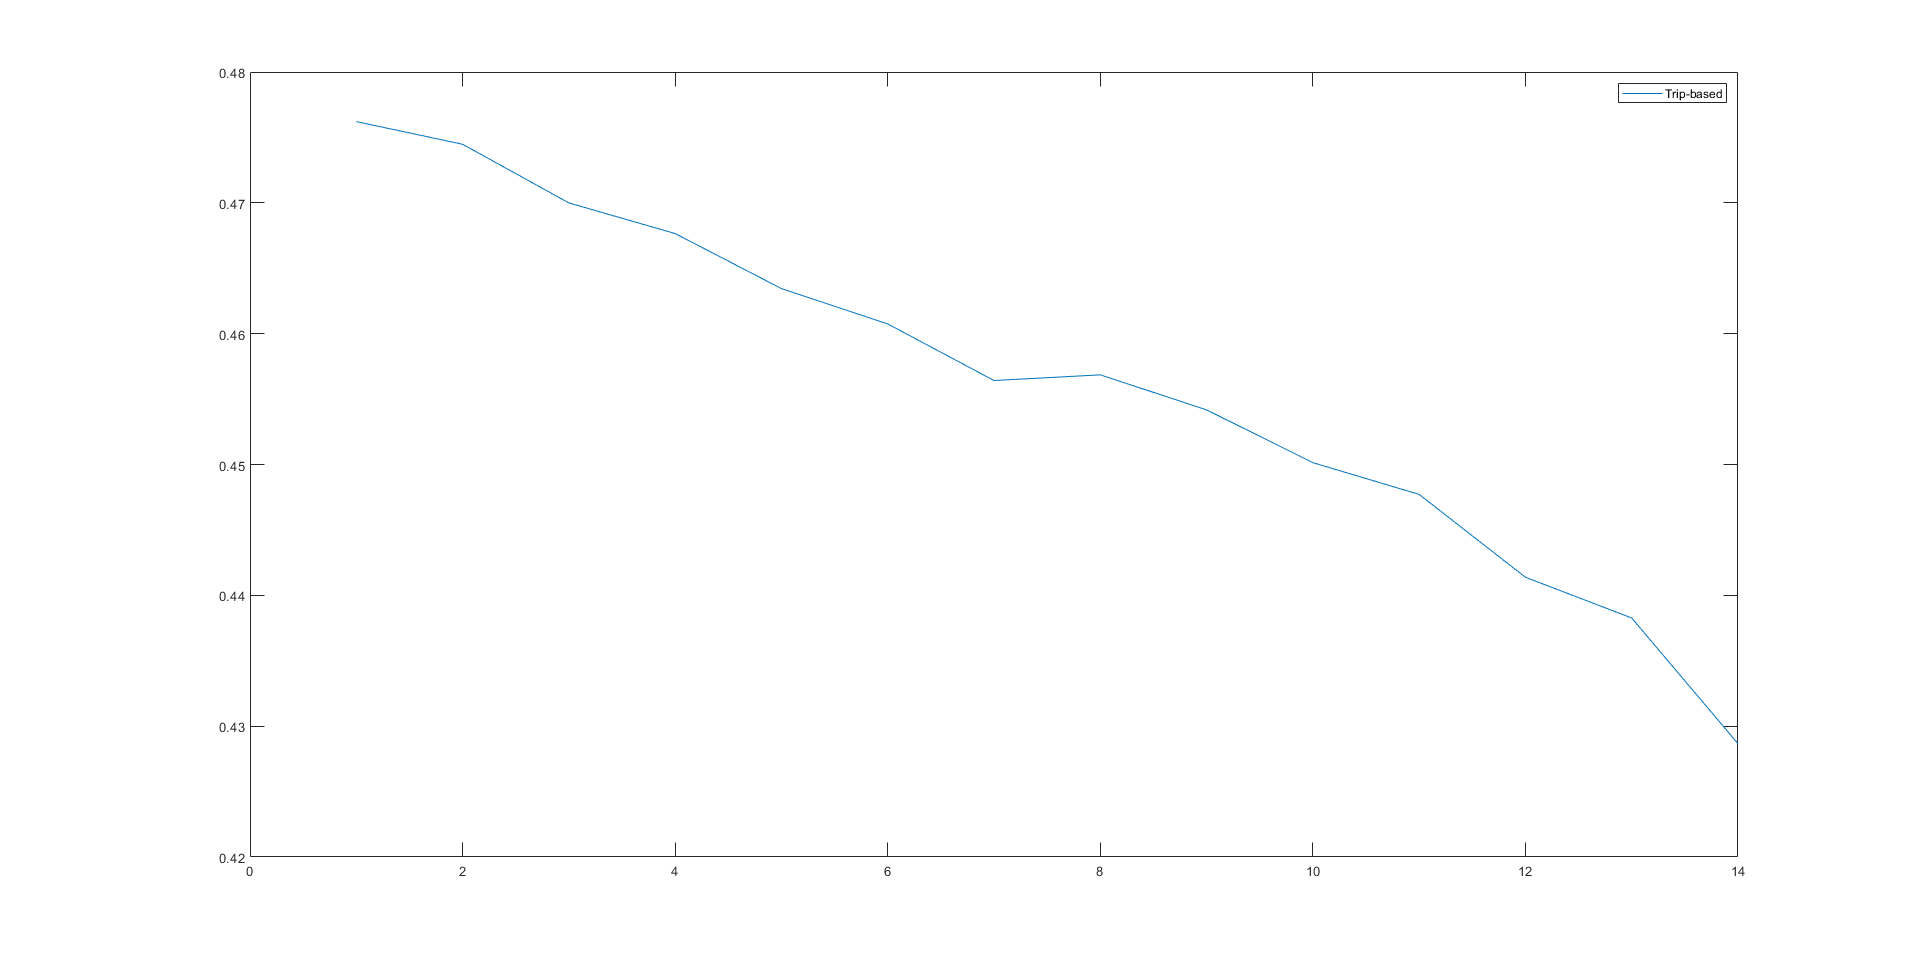
\includegraphics[width=1\textwidth]{figures/RMSN_chart.png}
  \caption{Results Of Munich trip-based calibration}
  \label{fig:munich-calibration}
\end{figure}

\section{Further improvements and other possible approaches}
\subsection{Vectorized operations}
An important factor to improve the performance of the current implementation of SPSA could be the use of vectorized operations in the code instead of for-loops while performing matrix multiplication operations. The advantage of such concept is that operations can be performed by a single command execution in a more efficient way. 

\subsection{Distributed computing}
A different approach in order to tackle the calibration limitations imposed by computational resources could be the usage of distributed technologies. By doing so, the processing loads of the calibration as well the simulations could be distributed among multiple machines working together. This can drastically improve the throughput and processing capacity of the approximation algorithm being used. 

\subsection{Gradient calculation}
Another interesting approach would be to use SPSA in combination with a different stochastic gradient descent (SGD) algorithm, such as Adam. The main idea in SGD algorithms, Adam for instance, is to make a bad estimate of the gradient of the loss (objective) function and take that gradient to move the model (in this case calibration) parameters in the desired direction. SPSA is quite similar, it makes a bad estimate of the gradient by performing the vector perturbations in both directions and adjusts the parameters of the calibration in the direction of the gradient. Similar to PC-SPSA, this could be a different approach that incorporates concepts being widely used at the moment in the context of deep learning and optimization problems.
